\section{Scaling Beyond Limits: Opportunities from Edge Devices}
\label{sec:opportunities}

\subsection{Massive Data from Edges}
\label{subsec:edge_data}

As discussed in §~\ref{subsec:data_exhaustion}, edge data represents a crucial alternative to synthetic data in addressing the challenge of data exhaustion. Edge data refers to the data generated by edge devices at or near the source of data generation, which typically remains private and localized rather than being publicly accessible. Edge devices encompass a wide range of equipment including Internet of Things (IoTs) sensors, smartphones, wearables, industrial controllers, and other smart devices that process data at the network edge. 
Data generated at edges offers unique advantages in both data volume and data quality. \looseness-1


\begin{figure*}[htbp]
    \centering
    \begin{minipage}[t]{0.49\linewidth}
        \centering
        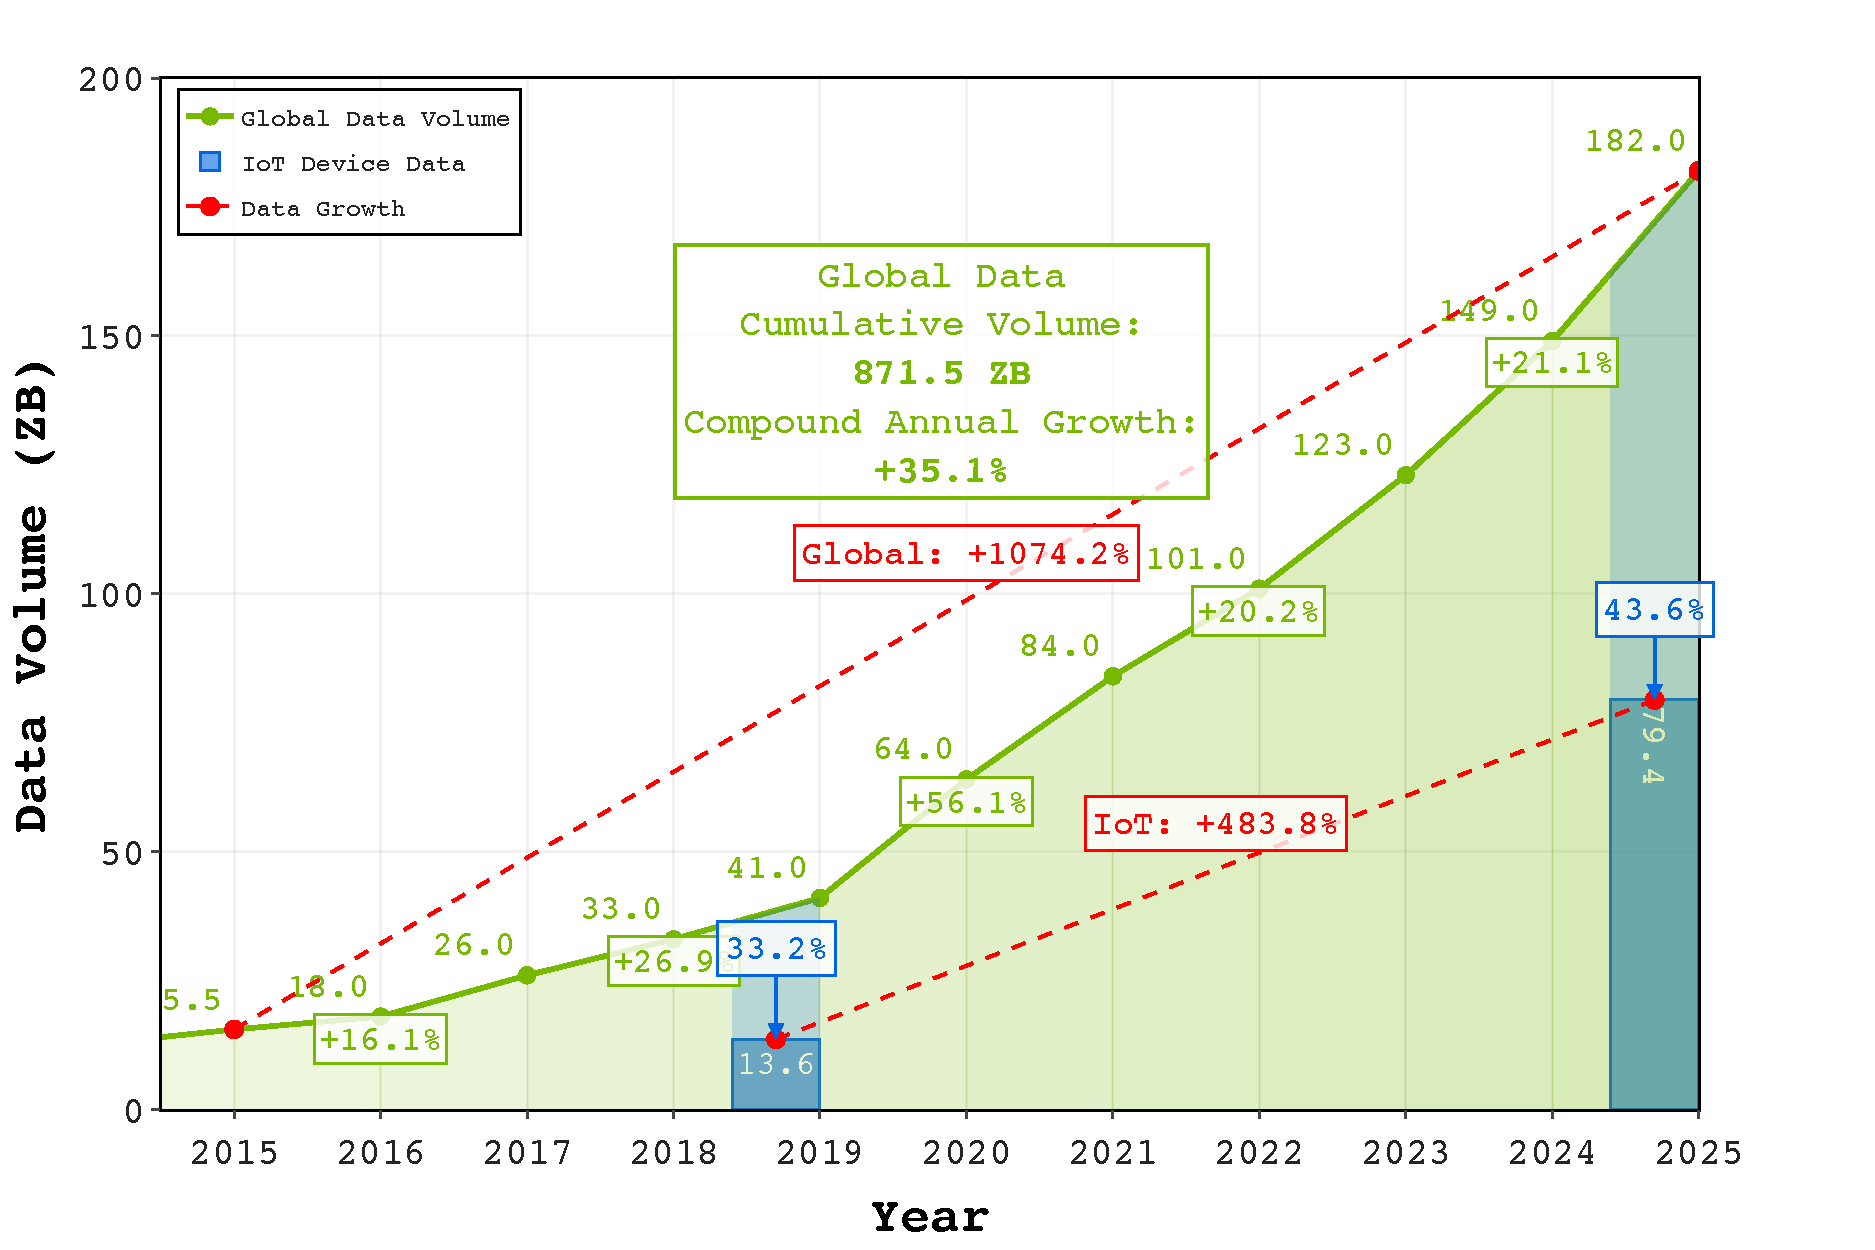
\includegraphics[width=\linewidth]{./figs/iot_data_contribution.pdf}
        % \vspace{-20pt}
        \caption{Global data volume from 2014 to 2025 and IoT device data volume in 2015 and 2025. (Data sources: Global data volume from \cite{statista_global_2023}; IoT device data volume from \cite{statista_iot_2023}.)}
    \label{fig:global_data}
    \end{minipage}
    \hfill
    \begin{minipage}[t]{0.49\linewidth}
        \centering
        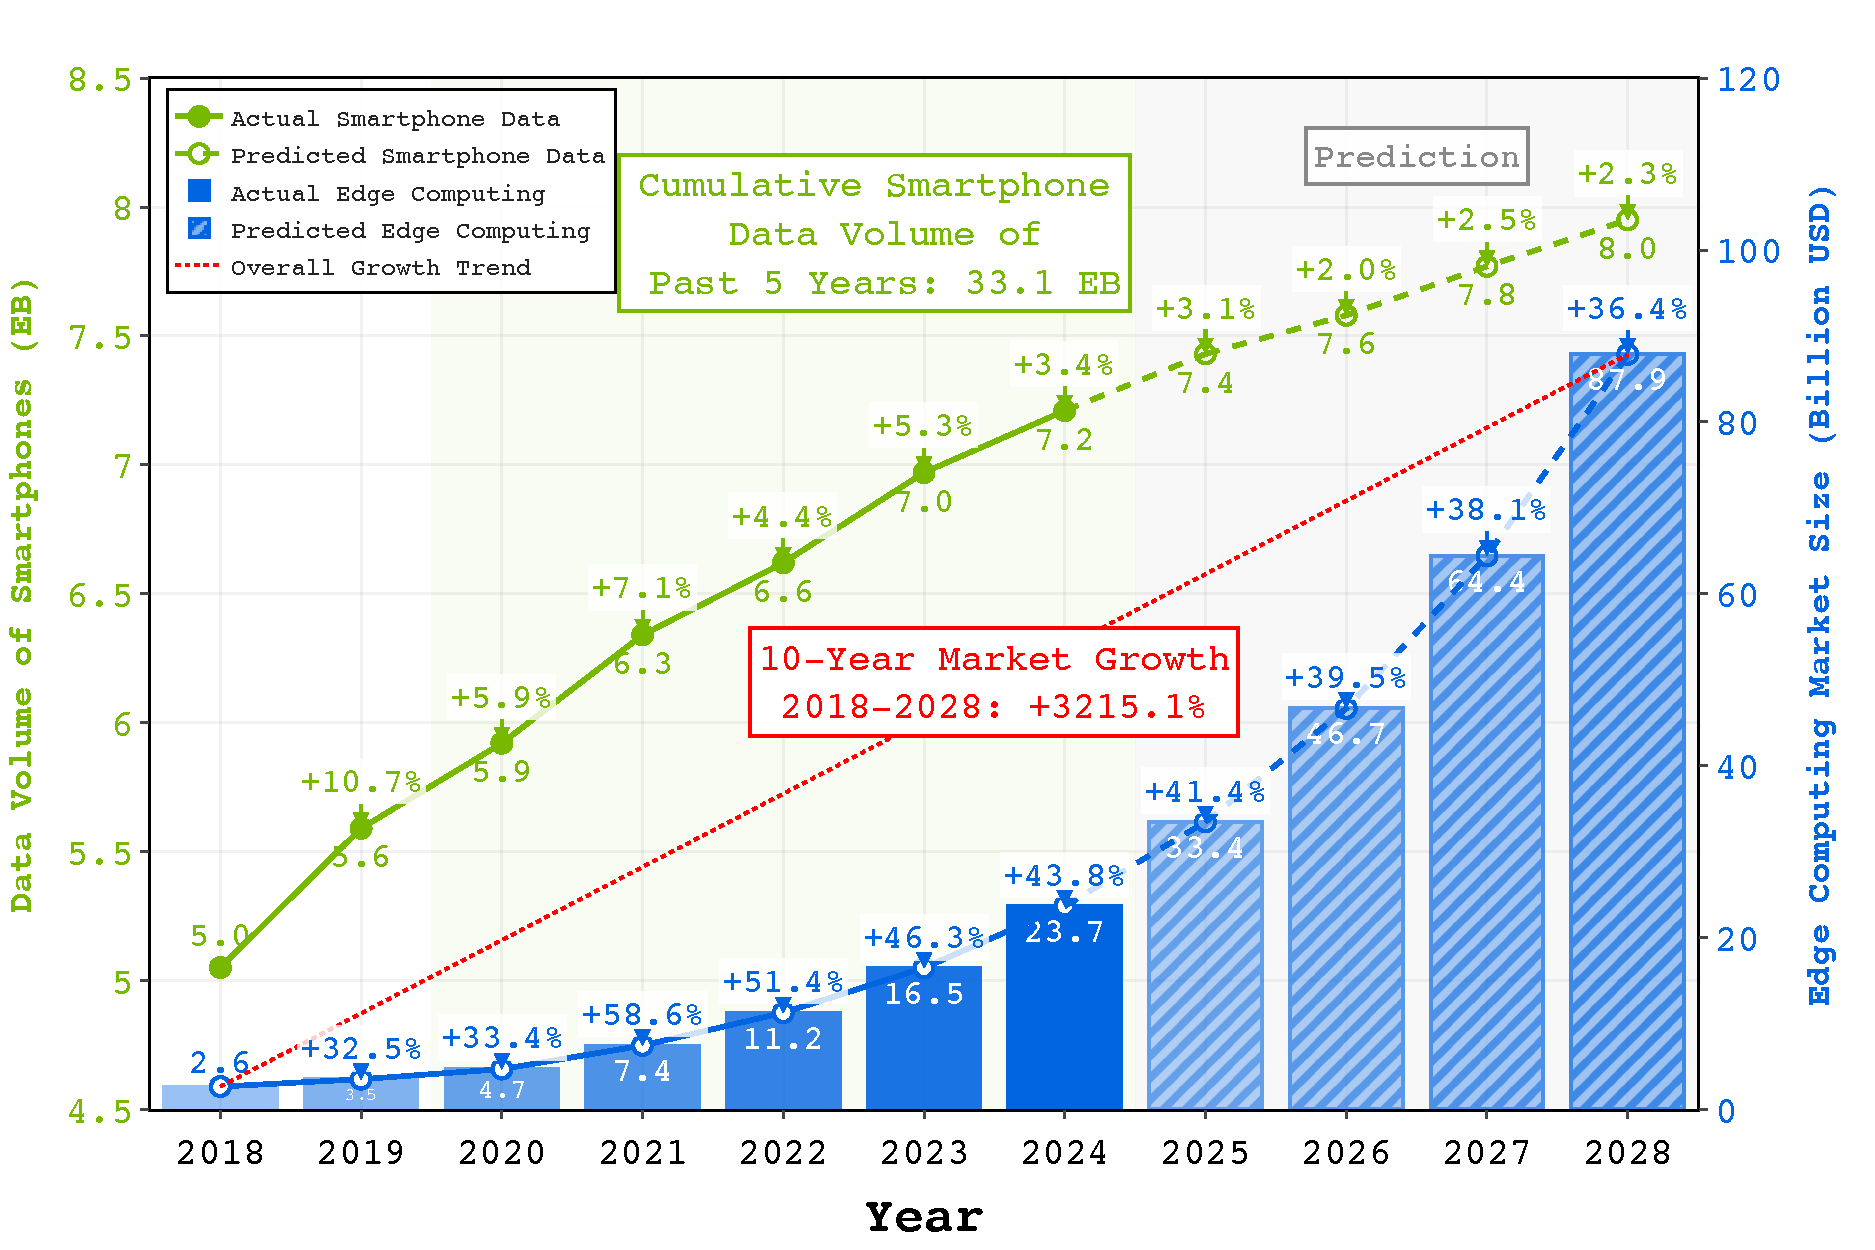
\includegraphics[width=\linewidth]{./figs/edge_and_smartphone.pdf}
        % \vspace{-20pt}

        \caption{Smartphone data volume with edge computing market size (right) from 2018 to 2028. (Data sources: Edge computing market \cite{grandview_edge_2023}; Smartphone data volume from \cite{bankmycell_smartphone_2023}.)}
    \label{fig:smartphone}
    \end{minipage}
    \vspace{-10pt}
\end{figure*}

\paragraph{Edge-generated data is explosively growing.} 
% By 2025, it is projected that over 80\% of global data will be generated directly at the edge, rather than in traditional centralized data centers \cite{seagate_rethinkdata_2020}. This shift highlights a fundamental transformation in how data is created, processed, and utilized across industries.
According to the statistical data from \cite{statista_global_2023,statista_iot_2023} (as illustrated in Figure~\ref{fig:global_data}), 
the global data volume is projected to reach 182 ZB by 2025~\cite{statista_global_2023}, where the data generated by IoT devices is anticipated to increase from 13.6 ZB in 2019 to 79.4 ZB in 2025~\cite{statista_iot_2023}, elevating its share of the global data volume from 33.2\% to 43.6\%, showing a particularly pronounced growth in edge-generated data. Over the period from 2015 to 2025, the global data volume exhibited a compound annual growth rate (CAGR) of 35.1\%, resulting in an overall increase of 1074.2\% and a cumulative total of 871.5 ZB. IoT device data experienced a growth of 483.8\% from 2019 to 2025. This trend underscores the increasingly central role of edge-generated data in the global data ecosystem.
Beyond IoT devices, smartphones, as a critical source of edge-side data, are also contributing to the steady rise in data volume. As depicted in Figure~\ref{fig:smartphone}, the estimated smartphone data volume is projected to grow from 5 EB in 2018 to 8 EB by 2028
\footnote{These numbers are estimated based on an average user data generation of 1 GB per device. For detailed estimation methodology, refer to Appendix \ref{app:smartphone_ethod}.}. 
This exponential growth is closely aligned with the rapid expansion of the edge computing market, which is forecasted to surge from \$5.5 billion in 2019 to \$87.9 billion by 2028, representing a remarkable growth rate of 3215.1\%. The burgeoning edge computing market has further catalyzed the generation and processing of edge-side data, reinforcing its significance in the broader data landscape 
\footnote{\cite{idc_seagate_dataage_2019,seagate_rethinkdata_2020} provide a more comprehensive overview of the global data volume, but we cannot access the statistics data. 
We appreciate any suggestions for better statistical data sources.
}.



\paragraph{Edge-generated data has distinctive advantages.} 
Beyond its impressive quantity, edge data possesses several distinctive characteristics that make it particularly valuable for model training.
First, edge data provides enhanced \textit{privacy} characteristics. Since edge data typically remains local to devices and does not need to be centrally stored, it allows for more privacy-preserving approaches to data utilization. This local-first nature enables compliance with increasingly strict data privacy regulations while still allowing the data to contribute to model training.
Second, edge data exhibits superior \textit{diversity} across multiple dimensions. It encompasses a wide variety of data types from IoT devices, mobile interactions, and personal devices, covering different domains, languages, and user behaviors. This natural diversity provides richer training signals compared to curated public datasets \cite{nayak2024review}. 
Third, edge data demonstrates strong \textit{real-time} capability. Unlike public datasets, which are often updated infrequently, edge devices continuously generate fresh data with low latency \cite{cavliwireless_edgecomputing}, offering more up-to-date and relevant training samples.
% Third, edge data offers enhanced \textit{personalization} characteristics. It enables real-time interactions and context-aware recommendations by leveraging local data such as location and device behavior. This allows for highly relevant and adaptive personalization that can dynamically adjust to user preferences \cite{xenonstack_edge_ai_2023}.
% Fourth, edge data exhibits enhanced \textit{context awareness} due to the proximal positioning of edge devices to data sources, enabling the capture of fine-grained contextual information often absent in public datasets. For instance, wearable devices collect synchronized activity and location data, providing high-fidelity behavioral patterns that preserve temporal and spatial context.
Despite these advantages, edge-generated data can present challenges such as low signal-to-noise ratios, unclean, or potentially harmful content. However, recent advancements in data quality assessment methods (e.g., data prospector \cite{ni2024small}), have emerged to identify and filter high-quality data from edge sources, ensuring that only the most reliable and valuable data is selected for model training.

In conclusion, edge data with its explosive growth and distinctive characteristics, is a valuable resource for model pretraining. Its diversity, real-time nature, personalization, and rich context make it an ideal foundation for developing robust and adaptable large-scale models, enhancing their ability to serve real-world applications effectively.

% \vspace{-0.5cm}
\begin{insights}
    \textbf{Insight:} The smartphone data volume of the past 5 years (before 2025) is projected to reach approximately 33.1 EB, with unique advantages in privacy, diversity, and real-time context, demonstrating the massive data potential of edge for AI model training.
\end{insights}
   



\subsection{Massive Computing Power from Edges}\label{subsec:edge_compute}



\paragraph{Edge computing power is growing rapidly.}
In recent years, edge computing has experienced explosive growth in computing power, driving smart devices to evolve from single-function tools into multimodal perception and decision-making centers. For instance, as shown in Figure~\ref{fig:edge_trend}, flagship smartphones such as the iPhone 16 series, equipped with 3nm process chips, have achieved computing power exceeding 2 TFLOPS~\cite{apple2024iphone16pro}, enabling local execution of complex AI tasks like real-time image enhancement and multilingual speech translation. 
Notably, the computing power of an individual smartphone has potentially surpassed that of laptops in the same period.
The breakthroughs are even more pronounced in the desktop sector,
% where NVIDIA's GeForce RTX 5090, with 104.9 TFLOPS of computing power~\cite{nvidia2025}, 
achieving an annual computing power growth rate of 1.29$\times$/year, surpassing that of smartphones and laptops (both 1.20$\times$/year). 
% \footnote{{Data source: \url{https://nanoreview.net}.}}
These three types of devices form a differentiated growth hierarchy, collectively driving edge computing's overall computing power to expand at an annual average rate of 1.28$\times$/year.
% , significantly outpacing the 1.3$\times$ growth rate of cloud computing~\cite{epoch2023trendsinmachinelearninghardware}, with the gap between the two continuing to narrow. 
This growth is fueled by three key technological drivers: advanced manufacturing processes (3nm technology increases transistor density by 60\%~\cite{apple2024iphone16pro}), dedicated architectures (modern smartphone SoCs integrate NPUs for AI acceleration), and scenario-driven innovation (e.g., autonomous driving demands end-to-end latency of less than 100ms~\cite{nvidia2023}).
% The quantitative increase in computational power has led to qualitative transformations: AR/VR devices can now reduce spatial modeling latency from seconds to milliseconds~\cite{idtechex2024}; medical-grade wearable devices can perform real-time analysis of 12-lead ECG data~\cite{gopala2022edge}; and educational tablets are capable of rendering 8K-resolution holographic teaching environments~\cite{precedence2024}. 
% These advancements have elevated edge computing from a supporting role to a core enabler of intelligence. The rapid growth of the global edge AI chip market~\cite{cognitive2024} further underscores the trend of computing power shifting toward the edge. 

\begin{figure*}[htbp]
    \centering
    \begin{minipage}[t]{0.49\linewidth}
        \centering
        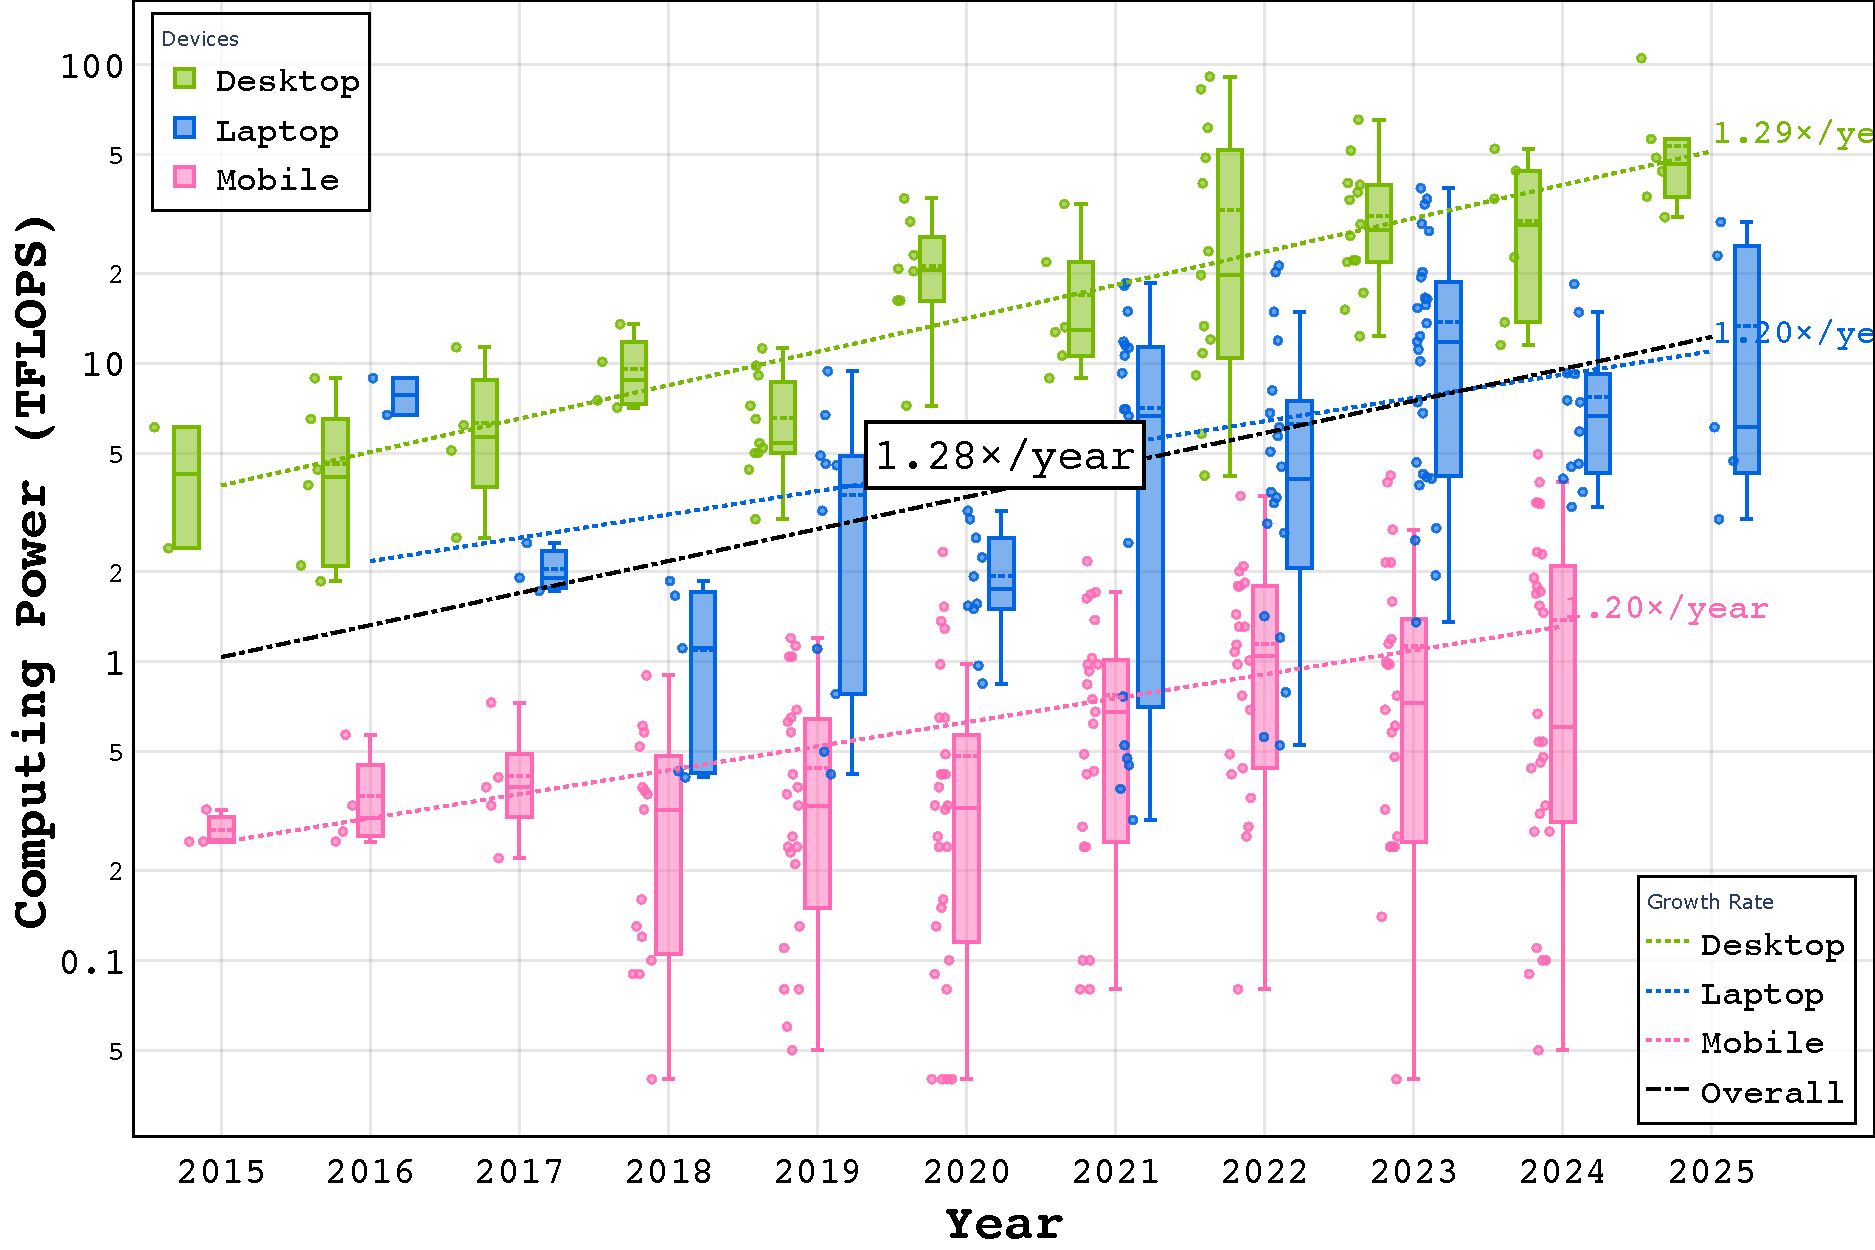
\includegraphics[width=\linewidth]{./figs/edge_compute_trend.pdf}
        % \vspace{-20pt}
        \caption{Edge Computing Power Evolution Trend. (Data source: \cite{nanoreview2025}).}
        \label{fig:edge_trend}
    \end{minipage}
    \hfill
    \begin{minipage}[t]{0.49\linewidth}
        \centering
        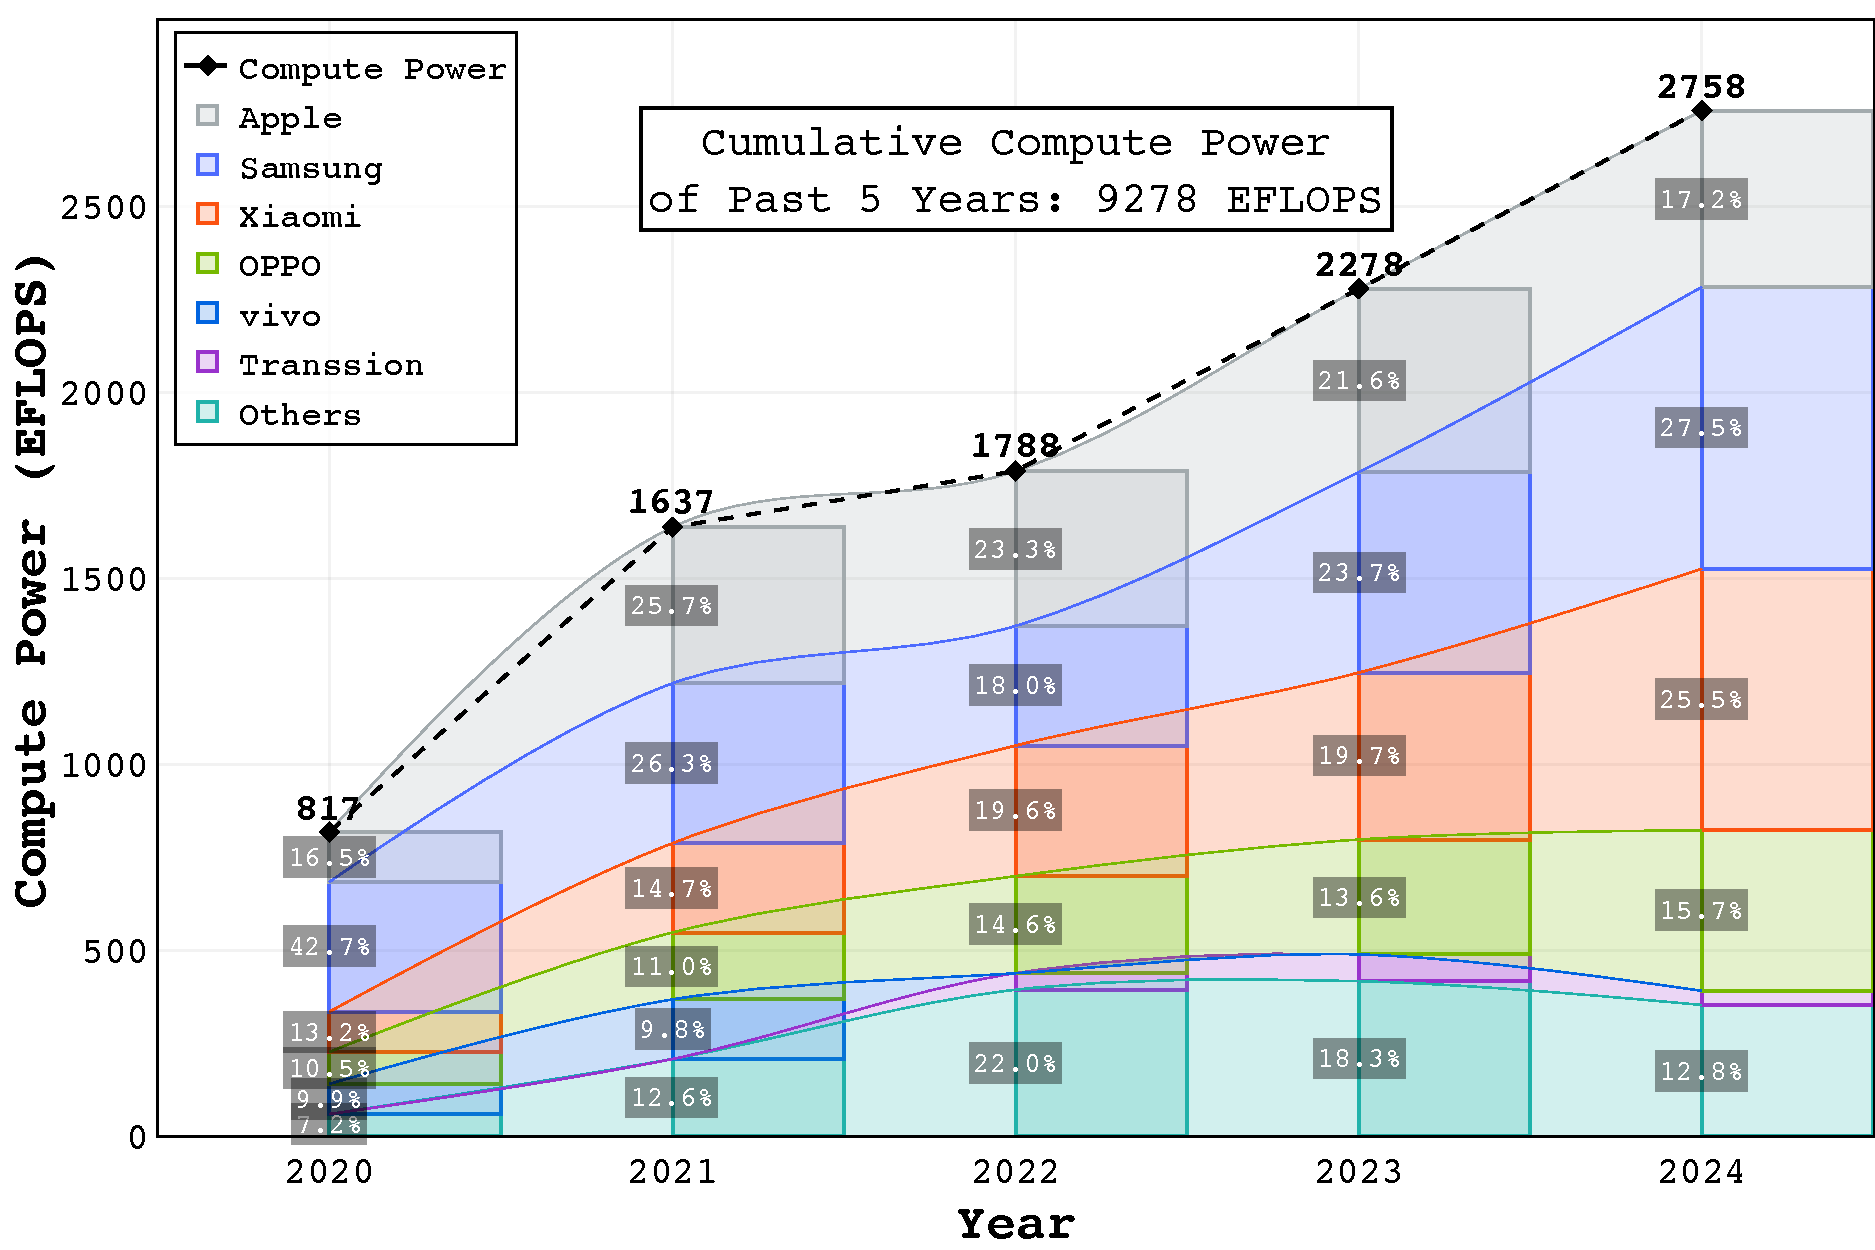
\includegraphics[width=\linewidth]{./figs/smartphone_compute_trend.pdf}
        % \vspace{-20pt}
        \caption{Smartphone Market Share and Computing Power Trends. (Data source: \cite{canalys2025}).}
        \label{fig:smartphone_trend}
    \end{minipage}
    \vspace{-10pt}
\end{figure*}


\paragraph{Edge computing has potential for LLM training.}
We analyze the performance of smartphone chips, representing typical edge devices, and estimated their overall computing power.
% , as summarized in Table~\ref{tab:chip_performance}. 
To ensure our estimation is as accurate as possible, we based our calculations on the market share data from \cite{canalys2025}.
We then estimated the total computing power of newly produced mobile devices by averaging the chip performance of each brand.
From 2020 to 2024, smartphone chip performance has seen significant improvements, with peak computing power increasing from 1.53 TFLOPS to 4.95 TFLOPS, and average computing power rising from 0.48 TFLOPS to 1.38 TFLOPS. Meanwhile, the overall computing power of mobile devices has grown from 817 EFLOPS in 2020 to 2,758 EFLOPS in 2024, and totally 9278 EFLOPS for past 5 years. This trend highlights the rapid expansion of edge computing power, which is not only essential for AI applications but also holds the potential for training complex AI models.
For instance, training the DeepSeek-v3~\cite{liu2024deepseek} model utilizes 2048 H100 GPUs, each providing a peak FP32 performance of 59.30 TFLOPS, resulting in a total computational capacity of 121,446.4 TFLOPS. If this workload were distributed across edge devices with a peak performance of 2 TFLOPS (e.g., mobile chips like the iPhone 16 series), approximately 60,723 users with edge devices working (\textit{ideally}) in parallel would be required to match the computational capacity. \looseness-1

\begin{insights}
    \textbf{Insight:} 
    The smartphone computing power of the past 5 years (before 2025) is projected to reach approximately 9278 EFLOPS, with individual flagship devices now achieving over 2 TFLOPS performance. The combined parallel computing power of approximately 30 iPhone devices (with A18 chips) can match the computational capacity of a professional AI training GPU (H100 with 59.30 TFLOPS). 
\end{insights}

However, current smartphone chips are primarily optimized only for inference efficiency rather than training capabilities. 
\textit{We advocate for and predict a future trajectory of edge computing where smartphone chip designs will increasingly prioritize and optimize on-device model training capabilities.
% , fundamentally transforming the edge computing landscape.
}
As computational power grows and distributed algorithms develop, we expect a paradigm shift enabling collaborative model training across networks of edge devices. This evolution positions the edge computing ecosystem as a critical catalyst for democratizing AI development and driving the next wave of innovations in the field.



